% !TeX spellcheck = it_IT
% !TeX root = ../../compl.tex
\section{Algoritmo di Karger per il taglio minimo}

Si consideri un grafo non orientato $G = (V,E)$. Una partizione $S, T \subseteq V$ dei vertici di $G$ (dunque $S \cap T \equiv \emptyset$ e $S \cup T \equiv V$) è detta \textit{ammissibile} se $S \not \equiv \emptyset$ e $T \not \equiv \emptyset$. Un \textit{taglio} in $G$ è un insieme $\Gamma (S, T) \equiv \left\{(u,v) \in E \mid u \in S, \ v \in T \right\}$ per una partizione ammissibile $S,T$ dei vertici di $G$ (i lati da "tagliare" nel grafo per dividerlo nei due insiemi che formano la partizione). In un grafo non pesato, il costo di un taglio corrisponde alla sua cardinalità $|\Gamma (S, T)|$.

In quanto segue consideriamo grafi non pesati e senza cappi; tuttavia, ammettiamo la presenza di archi multipli fra coppie di nodi (\textit{multigrafo}). In questo caso, $E$ è un multinsieme di archi, poiché archi fra coppie di vertici distinti possono essere presenti con molteplicità diverse.

\begin{figure}[ht!]
    \centering
    \resizebox{0.23\linewidth}{!}{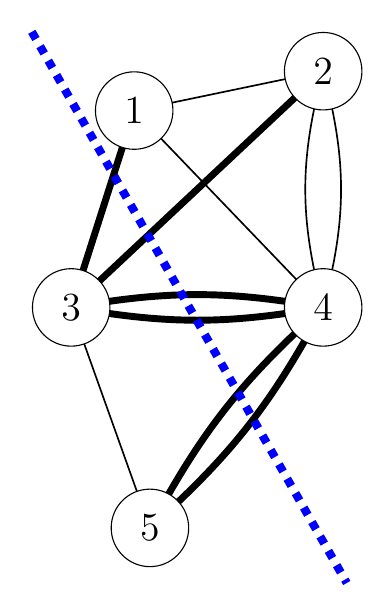
\begin{tikzpicture}[
    % Define Styles
    vertex/.style={
        circle,
        draw,
        minimum size=28pt,
        inner sep=0pt,
        fill=white,
        font=\Large\rmfamily
    },
    thickedge/.style={
        draw,
        line width=2.5pt
    },
    thinedge/.style={
        draw,
        semithick
    },
    cutline/.style={
        draw,
        blue,
        dashed,
        line width=3pt
    }
    ]

    % Define Coordinates
    \coordinate (c3) at (0, 0);       % Node 3 (Left Middle)
    \coordinate (c1) at (0.8, 2.5);   % Node 1 (Top Left)
    \coordinate (c2) at (3.2, 3.0);   % Node 2 (Top Right)
    \coordinate (c4) at (3.2, 0);     % Node 4 (Right Middle)
    \coordinate (c5) at (1.0, -2.8);  % Node 5 (Bottom)

    % Draw Edges

    % Edges connected to Node 1
    \draw[thinedge] (c1) -- (c2);
    \draw[thickedge] (c1) -- (c3);
    \draw[thinedge] (c1) -- (c4);

    % Edges connected to Node 2
    \draw[thickedge] (c2) -- (c3);
    % Double curved thin edges between 2 and 4
    \draw[thinedge] (c2) to[bend right=15] (c4);
    \draw[thinedge] (c2) to[bend left=15] (c4);

    % Edges connected to Node 3
    \draw[thickedge] (c3) to[bend right=10] (c4);
    \draw[thickedge] (c3) to[bend left=10] (c4);
    \draw[thinedge] (c3) -- (c5);

    % Edges connected to Node 4
    \draw[thickedge] (c4) to[bend right=10] (c5);
    \draw[thickedge] (c4) to[bend left=10] (c5);

    % Nodes
    \node[vertex] (n1) at (c1) {1};
    \node[vertex] (n2) at (c2) {2};
    \node[vertex] (n3) at (c3) {3};
    \node[vertex] (n4) at (c4) {4};
    \node[vertex] (n5) at (c5) {5};

    % Blue Cut Line
    \draw[cutline] (-0.5, 3.5) -- (3.5, -3.5);

\end{tikzpicture}}
    \caption{Un taglio in un multigrafo. Il taglio evidenziato è formato da 6 archi e corrisponde al multinsieme $\Gamma (S,T)$, dove $S = \left\{1,2,4\right\}$ e $T =\left\{3,5\right\}$}
\end{figure}


Il problema del taglio minimo (\textsc{MinCut}) su un multigrafo è definito nel modo seguente.
\boxProb{MinCut}
{Un multigrafo $G = (V,E)$}
{Una partizione ammissibile $S,T$ di $V$ che minimizza il costo $|\Gamma(S,T)|$}

Il problema MinCut ha tantissime applicazioni. Per esempio, in un sistema distribuito dove i nodi rappresentano i processi e gli archi canali di comunicazione fra di essi, il taglio minimo corrisponde ad assegnare i processi a due CPU in modo che la comunicazione inter-processore -- tipicamente lenta -- sia minimizzata. Una seconda applicazione è la segmentazione di immagini. Qui i nodi rappresentano pixel e gli archi del grafo connettono pixel simili. Il taglio minimo corrisponde allora a una segmentazione dell'immagine in due parti tra loro il più dissimili possibile.

Il problema MinCut è facilmente risolvibile in tempo polinomiale deterministico, per esempio usando l'algoritmo di \href{https://dl.acm.org/doi/pdf/10.1145/263867.263872}{\texttt{Stoer-Wagner}}, il quale ha un tempo di esecuzione dell'ordine $\O\left(|E||V| + |V|^2 \log |V|\right)$.

Mostriamo ora un semplice algoritmo probabilistico Monte Carlo, l'algoritmo di Karger, che trova il taglio minimo con probabilità almeno $1 - \epsilon$ in tempo pari a $\O\left(|E||V|^2 \log \frac{1}{\epsilon}\right)$.

\begin{figure}[ht!]
    \centering
    \resizebox{0.95\linewidth}{!}{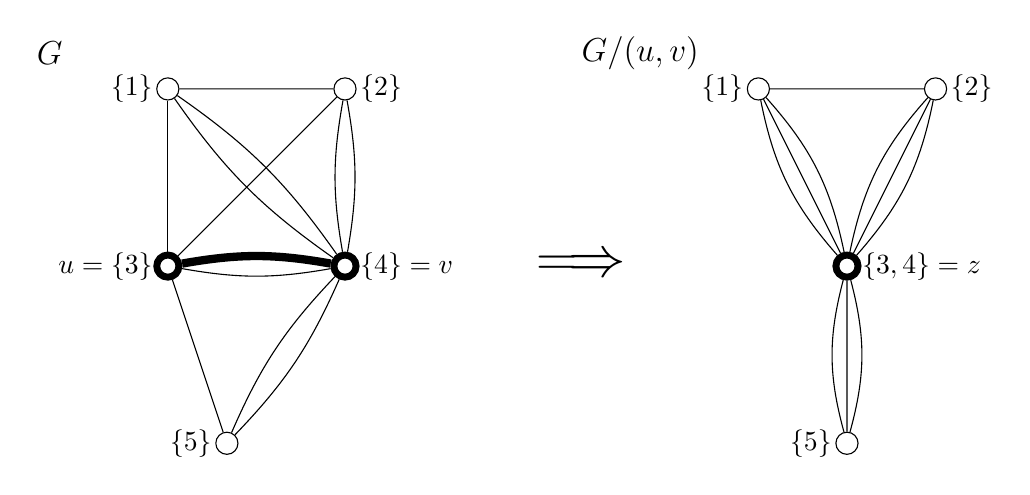
\begin{tikzpicture}[
    % Global styles
    vertex/.style={circle, draw=black, fill=white, inner sep=0pt, minimum size=8pt},
    boldvertex/.style={vertex, line width=2.5pt},
    scale=1.5  % Scaling up for better visibility
    ]
    % ===========================
    % LEFT GRAPH G
    % ===========================

    % Label G
    \node at (-1, 1.8) {\large $G$};

    % Nodes
    \node[vertex] (n1) at (0, 1.5) {};
    \node[vertex] (n2) at (1.5, 1.5) {};
    \node[boldvertex] (u) at (0, 0) {};
    \node[boldvertex] (v) at (1.5, 0) {};
    \node[vertex] (n5) at (0.5, -1.5) {};

    % Labels
    \node[left=2pt] at (n1) {$\{1\}$};
    \node[right=2pt] at (n2) {$\{2\}$};
    \node[left=2pt] at (u) {$u = \{3\}$};
    \node[right=2pt] at (v) {$\{4\} = v$};
    \node[left=2pt] at (n5) {$\{5\}$};

    % Edges
    % Top connections
    \draw (n1) -- (n2);
    \draw (n1) -- (u);
    \draw (n2) -- (u);
    \draw (n1) to[bend left=10] (v);
    \draw (n1) to[bend right=10] (v);

    % Multiple edges between 2 and v
    \draw (n2) to[bend right=10] (v);
    \draw (n2) to[bend left=10] (v);

    % Connection u-v (Thick line + 2 curves)
    \draw[line width=3pt] (u) to[bend left=10] (v);
    \draw (u) to[bend right=10] (v);

    % Bottom connections
    \draw (u) -- (n5);
    \draw (v) to[bend left=10] (n5);
    \draw (v) to[bend right=10] (n5);


    % ===========================
    % ARROW
    % ===========================
    \node at (3.5, 0) {\huge $\Longrightarrow$};


    % ===========================
    % RIGHT GRAPH G/(u,v)
    % ===========================

    % Shift coordinates by x=5
    \begin{scope}[shift={(5,0)}]

        % Label G/(u,v)
        \node at (-1, 1.8) {\large $G/(u, v)$};

        % Nodes
        \node[vertex] (rn1) at (0, 1.5) {};
        \node[vertex] (rn2) at (1.5, 1.5) {};
        % The contracted node z is roughly between where u and v were
        \node[boldvertex] (z) at (0.75, 0) {};
        \node[vertex] (rn5) at (0.75, -1.5) {};

        % Labels
        \node[left=2pt] at (rn1) {$\{1\}$};
        \node[right=2pt] at (rn2) {$\{2\}$};
        \node[right=2pt] at (z) {$\{3, 4\} = z$};
        \node[left=2pt] at (rn5) {$\{5\}$};

        % Edges
        % 1 to 2
        \draw (rn1) -- (rn2);

        % 1 to z
        \draw (rn1) to[bend left=15] (z);
        \draw (rn1) to[bend right=15] (z);
        \draw (rn1) -- (z);

        % 2 to z (3 edges)
        \draw (rn2) to (z);         % center
        \draw (rn2) to[bend left=15] (z);
        \draw (rn2) to[bend right=15] (z);

        % 5 to z (2 edges)
        \draw (rn5) to[bend left=15] (z);
        \draw (rn5) to[bend right=15] (z);
        \draw (rn5) -- (z);

    \end{scope}

\end{tikzpicture}}
    \caption{La contrazione di un arco in un multigrafo.}
    \label{fig:kargContr}
\end{figure}

L'algoritmo di Karger è basato sull'operazione di contrazione di un arco (vedi Figura \ref{fig:kargContr}). La \textit{contrazione} di un arco $(u,v)$ in un multigrafo $G$ produce un multigrafo $G \setminus (u,v)$ definito come risultato delle seguenti operazioni:
\begin{enumerate}
    \item Un nuovo vertice $z$ è aggiunto al grafo

    \item Ogni arco $(w,u) \in E$ con $w \neq v$ è sostituito da un arco $(w,z)$

    \item Ogni arco $(w,v) \in E$ con $w \neq u$ è sostituito da un arco $(w,z)$

    \item Gli archi del tipo $(u,v)$ e i vertici $u,v$ sono rimossi
\end{enumerate}

Nel seguito, diciamo che $z$ è un supervertice che contiene $u$ e $v$. Quando uno o entrambi i due vertici agli estremi di un arco contratto solo a loro volta supervertici, allora i nodi in essi contenuti diventano parte del nuovo supervertice.

Introduciamo ora l'algoritmo Karger "base", il quale contrae ripetutamente archi a caso del multigrafo  fino a quando il numero di supervertici rimanenti è pari a due. Dato che la contrazione di un arco riduce di uno il numero di supervertici, l'algoritmo si fermerà dopo esattamente $|V| - 2$ passi. A questo punto, l'algoritmo produce il cut corrispondente all'unica partizione ammissibile dei due supervertici (si tagliano gli archi che collegano i vertici rimanenti). Dato che i supervertici del multigrafo finale corrispondono a una partizione dei vertici del multigrafo iniziale (i due supervertici dividono in due il grafo iniziale), abbiamo ottenuto un taglio del multigrafo iniziale.

\begin{algorithm}
    \caption{Karger-Base$(G)$}
    \KwInput{Multigrafo $G =(V,E)$ con $|V| > 2$}
    \While{$|V| > 2$}{
        Scegli un arco a caso $(u,v) \in E$\;
        $G \leftarrow G \setminus (u,v)$
    }
    \KwOutput{l'unica partizione ammissibile $S,T$ rimasta in $G$}
\end{algorithm}

Questo algoritmo può essere implementato in tempo $\O(|E|)$ rappresentando la sequenza di contrazioni tramite una permutazione causale degli archi di $G$ (dettagli omessi).

Vediamo ora qual è la probabilità che questo algoritmo ritorni una partizione ammissibile $S^\ast, T^\ast$ fissata che definisce un taglio $\Gamma^\ast = \Gamma \left(S^\ast, T^\ast \right)$ di costo minimo $k$ in $G$; in particolare
$$ k = |\Gamma^\ast| = \min_{(S,T)} |\Gamma(S,T)| $$
dove il minimo è su tutte le partizioni ammissibili $S,T$ di $V$. Per prima cosa, si noti che l'algoritmo ritorna $\Gamma^\ast$ se e solo se nessun arco in tale taglio viene contratto. Denotiamo ora con $X_1, \dots, X_{|V| - 2}$ la sequenza di archi contratti dall'algoritmo. La probabilità che il primo arco $X_1$ contratto sia nel taglio corrisponde a
$$ \Pr (X_1 \in \Gamma^\ast) = \frac{k}{|E|} \leq \frac{k}{|V| k/2} = \frac{2}{|V|}$$
perché la cardinalità di $E$ è tale che
$$ |E| = \frac{1}{2} \sum_{v \in V} d_v \geq \frac{1}{2} |V| d_{\min} \geq \frac{1}{2} |V| k $$
dove $d_v$ è il grado di $v \in V$ in $G$, mentre $d_{\min}$ è il grado minimo dei nodi del grafo. In particolare, $d_{\min} \geq k$ è vero perché il costo $k$ di un taglio minimo è sicuramente non superiore rispetto al costo $d_v$ del taglio $\Gamma (\{v\}, V \setminus \{v\})$ per qualsiasi vertice $v \in V$. In altre parole, il numero di archi è sicuramente maggiore del numero di vertici moltiplicato per metà del grado minimo di qualsiasi vertice, e sappiamo che $d_{\min} \geq k$.

Quindi
$$ \Pr \left(X_1 \notin \Gamma^\ast\right) \geq 1 - \frac{2}{|V|} $$

La probabilità che il secondo arco contratto $X_2$ non sia nel taglio $\Gamma^\ast$, dato che $X_1 \notin \Gamma^\ast$, è
\begin{align*}
    \Pr (X_2 \notin \Gamma^\ast \mid X_1 \notin \Gamma^\ast) & = 1 - \Pr (X_2 \in \Gamma^\ast \mid X_1 \notin \Gamma^\ast) \\
    & \geq 1 - \frac{k}{(|V| - 1) k/2} \\
    & = 1 - \frac{2}{|V| - 1}
\end{align*}

In generale, denotando con $A_i$ l'evento $X_i \notin \Gamma^\ast$ per $i \geq 1$, osserviamo che nessun arco di $\Gamma^\ast$ è stato già contratto nel momento in cui dobbiamo scegliere $X_i$ se condizioniamo sugli eventi $A_1, \dots, A_{i-1}$. Il taglio $\Gamma^\ast$ è dunque preservato sotto questo condizionamento. In aggiunta, al passo $i$-esimo, il grafo presenta $|V| - i + 1$ (super)vertici e un suo taglio minimo avrà ancora costo $k$ condizionando su $A_1, \dots, A_{i-1}$: le contrazioni si limitano a restringere le scelte di partizioni ammissibili dei vertici su cui valutare il costo dei tagli, e sappiamo che $\Gamma^\ast$ è preservato.

Di conseguenza, abbiamo che
\begin{align*}
	\Pr \left(A_i \mid A_1, \dots, A_{i-1}\right) & \geq 1 - \frac{k}{(|V| - i + 1) k /2} \\ 
	& = 1 - \frac{2}{|V| - i + 1} \\
	& = \frac{|V| - i + 1 - 2}{|V| - i  + 1} \\
	& = \frac{|V| - i - 1}{|V| - i + 1} && (\dag)
\end{align*}

Dunque, indicando $\Pr(A_1 \mid A_0) = \Pr (A_1)$, dove $A_0$ corrisponde all'evento certo, possiamo scrivere
\begin{align*}
    \Pr (\text{restituisce } \Gamma^\ast) & = \Pr \left(X_i \notin \Gamma^\ast, \ \forall i \in \left[|V| - 2\right]\right) \\
    & = \Pr \left(\bigcap_{i=1}^{|V| - 2} A_i \right) \\
    & = \prod_{i=1}^{|V|-2} \Pr \left(A_i \mid A_0, \dots, A_{i-1} \right) \\
    & \geq \prod_{i=0}^{|V| - 3} \frac{|V| - i - 2}{|V| - i} && (\text{per } (\dag) \text{, sottraendo } 1) \\
    & = \frac{\prod_{i=1}^{|V| - 2} i}{\prod_{j=3}^{|V|} j} = \frac{\left(|V| - 2\right)!}{\frac{|V|!}{2!}} = \frac{1}{\binom{|V|}{2}} && (\dag \dag)
\end{align*}

Possiamo amplificare la probabilità di successo eseguendo più volte l'algoritmo e scegliendo la partizione ammissibile che minimizza il costo del taglio tra tutte quelle ottenute. In particolare, se $M$ è un numero sufficientemente grande, allora siamo in grado di ottenere un taglio di costo minimo in una delle $M$ esecuzioni indipendenti dell'algoritmo con probabilità almeno $1 - \epsilon$, data una probabilità massima di errore $\epsilon \in (0,1]$. Questa idea viene implementata nell'algoritmo seguente.

\begin{algorithm}
    \caption{Karger$(G, \epsilon)$}
    \KwInput{Multigrafo $G = (V,E)$ con $|V| > 2$, parametro di confidenza $\epsilon \in (0,1]$}
    $M \leftarrow \left\lceil \binom{|V|}{2} \ln \frac{1}{\epsilon} \right\rceil$\;
    \For{$i = 1, \dots, M$}{
        $S_i, T_i \leftarrow$ Karger-Base$(G)$\;
    }
    $j \in \arg \min_{i = 1, \dots, M} |\Gamma \left(S_i, T_i\right)|$\;
\end{algorithm}

Ripetendo l'algoritmo base per $M = \left\lceil \binom{|V|}{2} \ln \frac{1}{\epsilon} \right\rceil = \O\left(|V|^2 \ln \frac{1}{\epsilon}\right)$ volte e scegliendo un taglio di costo minimo tra quelli prodotti, la probabilità che questo non abbia costo ottimo è
\begin{align*}
    \Pr \left(\text{Karger}(G, \epsilon) \text{ fallisce}\right) & = \Pr \left(|\Gamma (S_i, T_i)| > k, \ \forall i \in [M]\right) && \text{(nessun taglio output è minimo)} \\
    & \leq \Pr \left(\Gamma (S_i, T_i) \not \equiv \Gamma^\ast, \ \forall i \in [M]\right) && (\text{nessun taglio prodotto è } \Gamma^\ast) \\
    & = \Pr \left(\text{Karger-Base}(G) \text{ non restituisce } \Gamma^\ast \right)^M && (\text{indipendenza}) \\
    & = \left(1 - \frac{1}{\binom{|V|}{2}}\right)^M && (\text{per } (\dag \dag)) \\
    & \leq e^{- \frac{1}{\binom{|V|}{2}} M} && (1 - x \leq e^{-x}) \\ 
    & = e^{-\ln\frac{1}{\epsilon}} = \epsilon
\end{align*}
dove abbiamo usato la maggiorazione $1 - x \leq e^{-x}$ per ogni $x \in \R$. 

Il tempo totale di esecuzione, considerando anche il costo di ciascuna contrazione, è quindi $\O \left(|E| |V|^2 \ln \frac{1}{\epsilon}\right)$, dove
\begin{itemize}
	\item tempo $\O(|E|)$ per ogni ripetizione
	
	\item numero di ripetizioni $M =  \left\lceil \binom{|V|}{2} \ln \frac{1}{\epsilon} \right\rceil = \O \left(|V|^2 \ln \frac{1}{\epsilon} \right)$
\end{itemize}

Una versione più sofisticata, nota come \href{https://en.wikipedia.org/wiki/Karger%27s_algorithm#Karger%E2%80%93Stein_algorithm}{\texttt{algoritmo di Karger-Stein}}, trova un taglio di costo minimo con probabilità almeno $1 - \epsilon$ in tempo $\O \left(\left(|V|\ln|V|\right)^2 \ln \frac{1}{\epsilon}\right)$.
